\section{Fragen zu Vorlesung 2}
\subsection{Wie kommt man zu den verbundenen Dokumenten einer Richtlinie?}
Über das Amtsblatt der EU

\subsection{Wie läuft ein CE Konformitätsprozess zur Interverkehrbringung eines Produktes im europäischen Handelsraum aus?}

\begin{figure}[ht]
  \centering
  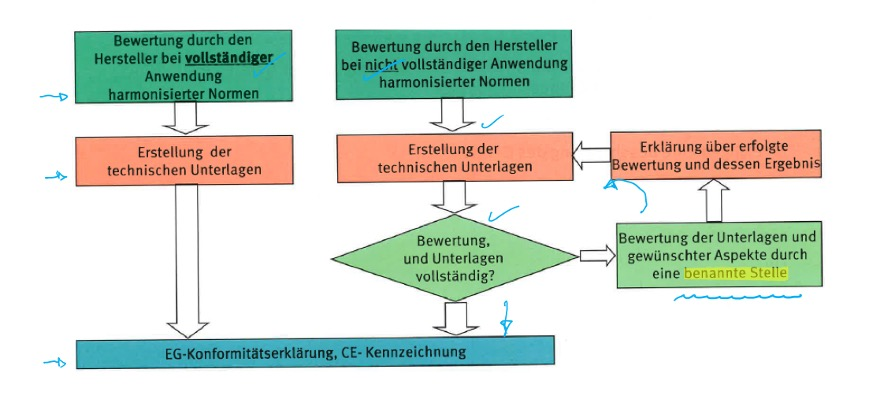
\includegraphics[height=7cm]{src/assets/pictures/lv2_konformitaetsprozess.jpg}
  \caption{Konformitätsbewertungsverfahren}
\end{figure}

\subsection{Was bedeutet das CE Zeichen?}
\begin{itemize}
  \item Das Produkt entspricht \textbf{allen} anzuwendenden Gemeinschaftsvorschriften
  \item Die entsprechenden Konformitätsbewertungsverfahren wurden durchgeführt
  \item Die Mitgliedstaaten dürfen das Inverkehrbringen nicht verhindern (außer das Produkt ist nicht konform)
  \item CE sagt nichts über die Herkunft des Produkts aus
\end{itemize}

\subsection{Dürfen Produkte ohne CE Zeichen in Europa in den Verkehr gebracht werden?}
\textbf{Ja}. Grundsätzlich brauchen Produkte, alle Produkte, die in der EU in Verkehr gebracht werden ein CE Kennzeichen.\p
Die Ausname machen hier ortsfeste Anlagen.

\subsection{Wer haftet wenn Geräte mit CE Zeichen umgebaut werden (müssen) z.B. -Änderung der Sendeantenne eines zertifizierten WLAN Moduls?}
Wenn ein CE gekennzeichnetes Gerät umgebaut und auf den Markt gebracht wird haftet immer derjenige, welcher das Gerät umgebaut hat.

\subsection{Begriffe im Sinne der EMV 2014/30/EU Richtlinie}
\subsubsection{Was ist ein Inverkehrbringer?}
Der Inverkehrbringer ist derjenige, welcher das Produkt auf dem Markt bereitstellt.

\subsubsection{Was ist ein Hersteller?}
Der Hersteller bringt das Gerät in Verkehr. Sie geben Namen, ihren eingetragenen Handlesnamen oder ihre eingetragene Handelsmarke und ihre Postanschrift entweder auf dem Gerät selbst, auf der Verpackung oder in den dem Gerät beigefügten Unterlagen an.

\subsubsection{Was ist ein Gerät?}
Ein fertiger Apparat oder eine als Funktionseinheit in den Handel gebrachte Kombination solcher Apparate, der bzw. die für den Endnutzer bestimmt ist/sind. Ein Gerät kann elektromagnetische Störungen verursachen oder durch sie beeinträchtigt werden.

\subsubsection{Was ist eine Anlage?}
Eine Anlage ist eine besondere Kombination von Geräten unterschiedlicher Art und gegebenenfalls weiteren Einrichtungen, die miteinander verbunden oder installiert werden.\p
Ist die Anlage dazu bestimmt auf Dauer an einem vorbestimmten Ort betrieben zu werden heißt sie \textbf{ortsfest}

\subsubsection{Was ist eine benannte Stelle?}
Staatlich benannte und staatlich überwachte private Prüfstellen.\p
Sie werden von der Kommission in einer Liste im Amtsblatt der EU veröffentlicht.

\subsection{Was passiert mit Geräten die ein CE Zeichen besitzen, nicht den Richtlinien entsprechen und trotzdem am Markt sind?}
Es werden alle zweckdienlichen Maßnamen ergriffen um das Gerät vom Markt zu nehmen, die Inverkehrbringung oder Inbetriebnahme zu untersagen oder den freien Verkehr für diese Gerät einzuschränken (EU-Weite Rückrufaktionen).

\subsection{Was ist eine Konformitätserklärung? Wer muss diese erstellen?}
Eine EU-Konformitätserklärung ist ein \textbf{zwingend notwendiges Dokument}, das entweder Sie als Hersteller oder Ihr bevollmächtigter Vertreter unterschreiben müssen, und mit dem Sie erklären, dass Ihre Produkte den EU-Anforderungen entsprechen. Mit der Unterzeichnung der Konformitätserklärung übernehmen Sie die volle Verantwortung dafür, dass Ihr Produkt dem geltenden EU-Recht entspricht.

\subsection{Wer haftet, bei Verletzung einer CE Erklärung?}
Es haftet derjenige, der die Konformitätserklärung unterzeichnet hat (Hersteller oder seine bevollmächtigten Vertreter).

\pagebreak